\section{Antenna Design 1 -- Monopole}
\label{sec:techsol1_monopole}
\begin{figure}[htbp]
    \begin{subfigure}[b]{0.49\linewidth}
        \centering
        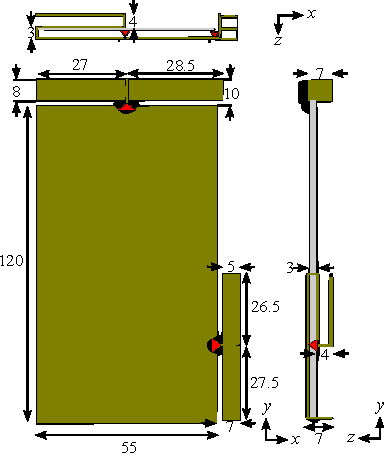
\includegraphics{img/tech_sol/monopole/tech_drawing}
        \caption{Technical drawing.}
        \label{fig:ant1technical}
    \end{subfigure}
    \hfill
    \begin{subfigure}[b]{0.49\linewidth}
        \centering
        \includegraphics{img/tech_sol/schematic_tuning_1}\\[1cm]
\footnotesize
        \begin{tabular}{|l|l|l|l|}
            \hline
            & $C_1$ & $L_1$ & $C_2$ \\
            \hline
            Top antenna & \SI{3.02}{pF} & \SI{7.99}{nH} & $[0.3,2.9]\,$pF\\
            Side antenna & \SI{1.81}{pF} & \SI{5.27}{nH} & $[0.3,2.9]\,$pF\\
            \hline
        \end{tabular}
        \caption{Tuning/matching circuit.}
        \label{fig:ant1_tuning}
    \end{subfigure}
    \caption{Technical drawing and tuning circuit for the antenna.  The matching circuit is applied for both the top and the side antenna.}
    \label{fig:ant1techschem}
\end{figure}

%Single antenna description
The antenna design for both antennas is shown in Figure \ref{fig:ant1technical}. Both antennas is designed from a basic folded monopole structure with 2 arms one for the low band and one for the high band. The antennas are almost identical with a few changes as a result of the restrictions on the ground clearance.
The antennas are designed to take full advantage of the ground clearance requirements in all directions. This is done in order to obtain the highest possible bandwidth in the low band and high band. 

%MIMO
Going from the top antenna to the side antenna the ground clearance decreases from \SI{10}{mm} to \SI{7}{mm}. To compensate for the decrease in ground clearance the length of both the low band and high band arms are adjusted to obtain the highest bandwidth within the low band and high band. 

The surface currents of the top antenna are shown in Figure \ref{fig:ant1_sc}. In the low band the left arm is excited and as the frequency increases the short becomes more excited. This illustrated the different operation modes and the of the two arm folded monopole.

The S-parameter for both antennas can be seen on Figure \ref{fig:ant1_sparam}. Both antennas are simulated with the tuning capacitors at \SI{0.3}{pF}. At this state both antennas covers the highest frequencies in the low- and highband. From the figure it can be seen that both antennas almost covers the entire high band. However some tuning is needed for the side antenna in the lower band.   

\begin{figure}[htbp]
   \begin{subfigure}[b]{0.32\linewidth}
        \centering
        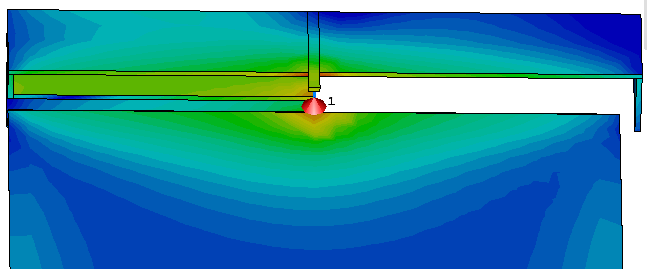
\includegraphics[width=\linewidth]{img/tech_sol/monopole/sc_800}
        \caption{Surface current for \SI{800}{MHz}}
        \label{fig:ant1_sc800}
    \end{subfigure}
    \hfill
    \begin{subfigure}[b]{0.32\linewidth}
        \centering
        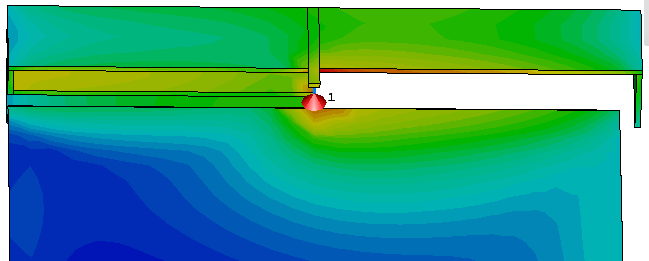
\includegraphics[width=\linewidth]{img/tech_sol/monopole/sc_1800}
        \caption{Surface current for \SI{1800}{MHz}}
        \label{fig:ant1_sc1800}
    \end{subfigure}
    \hfill
    \begin{subfigure}[b]{0.32\linewidth}
        \centering
        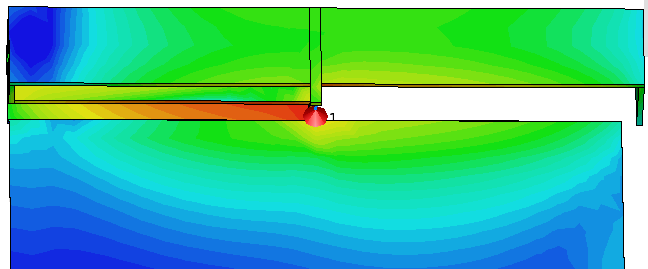
\includegraphics[width=\linewidth]{img/tech_sol/monopole/sc_2400}
        \caption{Surface current for \SI{2400}{MHz}}
        \label{fig:ant1_sc2400}
    \end{subfigure}
    \caption{Surface currents at each resonance with $C_2=\SI{0.3}{pF}$.}
    \label{fig:ant1_sc}
\end{figure}

\begin{figure}[htbp]
    \centering
    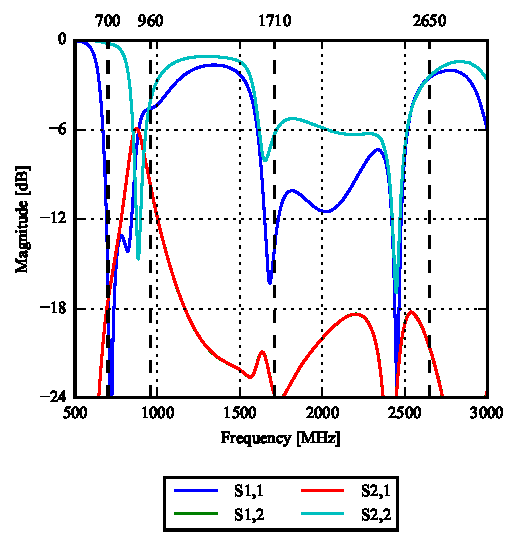
\includegraphics{img/tech_sol/monopole/ant1_sparam}
    \caption{S-parameters with $C_2=\SI{0.3}{pF}$ for both antennas.}
    \label{fig:ant1_sparam}
\end{figure}
The tuned S-parameters for both antennas are shown in Figure \ref{fig:sparam_mono_free_space}. The return loss $S_{11}$ and $S_{22}$ shows that both antennas almost covers the desired bandwidth. However from \SI{2500}{MHz} to \SI{2650}{MHz} both antennas are \SI{-1}{dB} to \SI{-3}{dB} lower than required. The side antenna \ref{fig:ant1_s22} also shows a lower level than desired at \SI{1750}{MHz} and in the low band limits. During the S-parameter simulation sweep of one antenna the variable capacitor of the other antenna is set to initial fixed value of \SI{0.3}{pF}. 

The isolation loss $S_{21}$ is shown in Figure \ref{fig:sparam_mono_free_space}. The $S_{21}$ sweep shows a low isolation loss at \SI{5}{dB} in the low band. The surface current simulations \ref{fig:ant1_sc} shows that the monopole antenna design excites the ground plane, which could cause the low isolation loss. This should be taken into consideration as the isolation loss can have a significant effect on the MIMO operation.      

The channel bandwidth for both antennas are shown in Table. \ref{tab:bw_sol1}. Both antennas have the desired bandwidth in the lower bands, however only the top antenna fulfill the bandwidth requirement in the high band. The side antenna lacks \SI{37}{MHz} in the high band.

%Correlation
The correlation between the antennas are shown in Figure \ref{fig:corr_sol1}. The Figure shows the correlation when sweeping the tuning capacitors from \SI{0.3}{pF} to \SI{2.9}{pF}m. From the figure it is seen that the correlation exceeds the requirement of \num{0.5} in the low band for both the top and side antenna with a maximum at \SI{700}{MHz}. The surface current at the different operation frequencies \ref{fig:ant1_sc} shows a strong coupling to the ground plane, which could cause the high correlation in the low band. 

%Efficiency
The efficiency for both antennas is shown in Figure \ref{fig:eff_sol1_free}. The efficiency is plotted for each sweep of the tunable capacitors. The efficiency mostly covers the entire spectrum with an efficiency of \SI{-3}{dB} with a drop of \SI{1.5}{dB} around \SI{750}{MHz} for the side antenna. 

    \begin{table}
        \centering
        \begin{tabular}{|l|l|r|r|r|}
            \hline
            Antenna & Band & Start [MHz] & Stop [MHz] & Bandwidth [MHz] \\
            \hline
            Top     & Low  & 680         & 1011       & 331 \\
            Side    & Low  & 818         & 909        & 91 \\
            \hline
            Top     & High & 1590        & 2527       & 937 \\
            Side    & High & 1850        & 2533       & 683 \\
            \hline
        \end{tabular}
        \caption{Maximum bandwidth obtained in the low and high band for the top and the side antenna, respectively.}
        \label{tab:bw_sol1}
    \end{table}

%S-Parameter sweep
\begin{figure}[htbp]
   \begin{subfigure}[b]{0.49\linewidth}
        \centering
        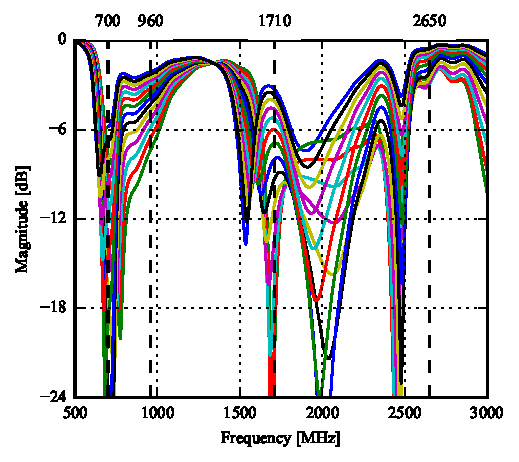
\includegraphics{img/tech_sol/monopole/s11}
        \caption{$S_{11}$, sweeping $C_1$ and fixing $C_2$.}
        \label{fig:ant1_s11}
    \end{subfigure}
    \hfill
    \begin{subfigure}[b]{0.49\linewidth}
        \centering
        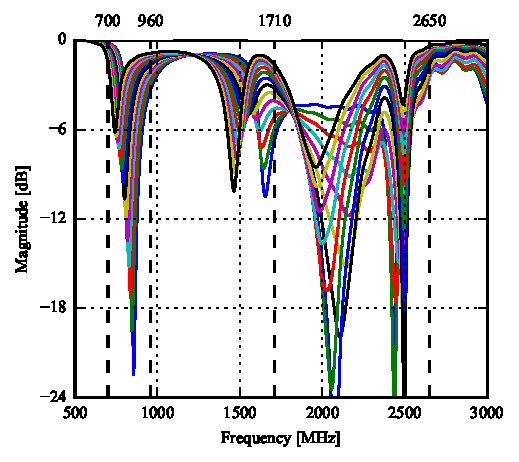
\includegraphics{img/tech_sol/monopole/s22}
        \caption{$S_{22}$, sweeping $C_2$ and fixing $C_1$.}
        \label{fig:ant1_s22}
    \end{subfigure}
~
    \begin{subfigure}[b]{0.49\linewidth}
        \centering
        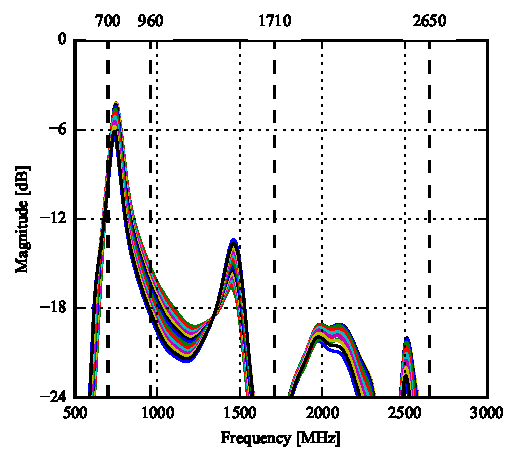
\includegraphics{img/tech_sol/monopole/s21-s11}
        \caption{$S_{21}$, sweeping $C_1$ and fixing $C_2$.}
        \label{fig:ant1_s11}
    \end{subfigure}
    \hfill
    \begin{subfigure}[b]{0.49\linewidth}
        \centering
        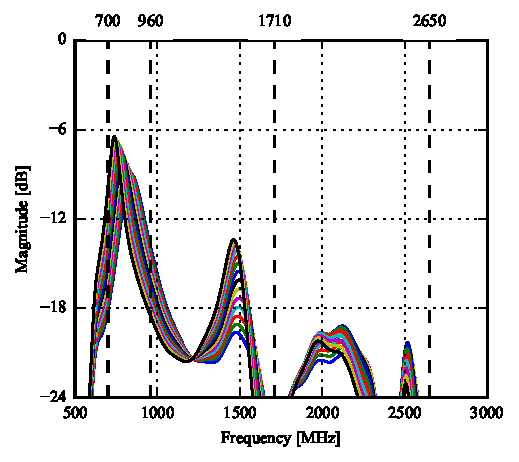
\includegraphics{img/tech_sol/monopole/s21-s22}
        \caption{$S_{21}$, sweeping $C_2$ and fixing $C_1$.}
        \label{fig:ant1_s22}
    \end{subfigure}
    \caption{S-parameter sweep in free space for tuning the shunt capacitor of each antenna, $C_1$ and $C_2$ for port 1 and 2, respectively. Port 1 is the top antenna and port 2 is the side antenna.}
    \label{fig:sparam_mono_free_space}
\end{figure}

% Correlation
\begin{figure}[htbp]
    \centering
    \begin{subfigure}{0.49\linewidth}
        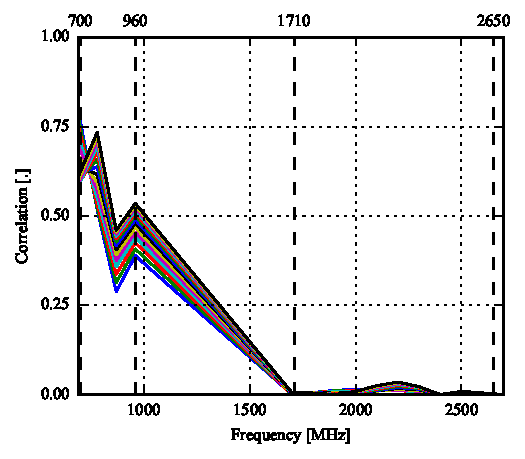
\includegraphics{img/tech_sol/monopole/free_space/s11_corr}
        \caption{Sweeping $C_1$ and fixing $C_2$.}
    \end{subfigure}
    \hfill
    \begin{subfigure}{0.49\linewidth}
        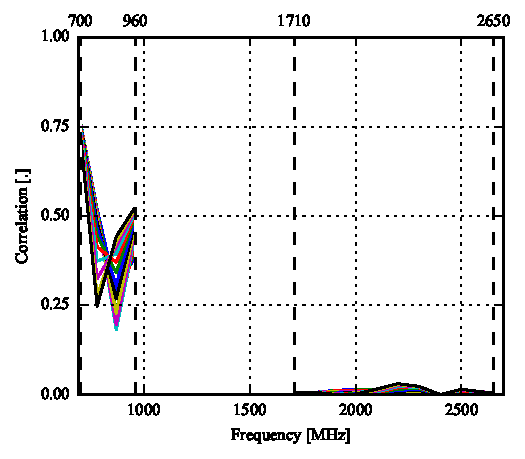
\includegraphics{img/tech_sol/monopole/free_space/s22_corr}
        \caption{Sweeping $C_2$ and fixing $C_1$.}
    \end{subfigure}
    \caption{Correlation between antennas when sweeping tuning capacitors. Here, $C_1$ and $C_2$ are the tuning capacitor for the top and side antenna, respectively.}
    \label{fig:corr_sol1}
\end{figure}

\begin{figure}[htbp]
    \centering
    \begin{subfigure}{0.49\linewidth}
        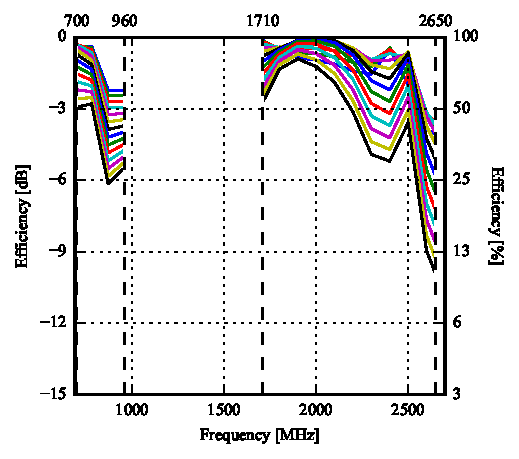
\includegraphics{img/tech_sol/monopole/free_space/efficiency-ac1-csh1}
        \caption{Sweeping $C_1$ and fixing $C_2$.}
    \end{subfigure}
    \hfill
    \begin{subfigure}{0.49\linewidth}
        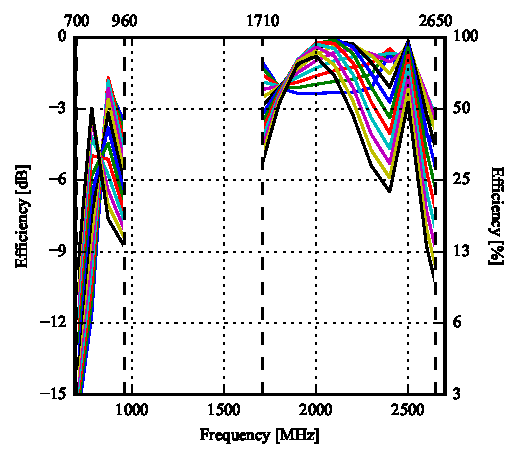
\includegraphics{img/tech_sol/monopole/free_space/efficiency-ac2-csh2}
        \caption{Sweeping $C_2$ and fixing $C_1$.}
    \end{subfigure}
    \caption{Monopole antenna in free space. Efficiency for each antenna when sweeping the tunable capacitors. Here, $C_1$ and $C_2$ are the tuning capacitor for the top and side antenna, respectively.}
    \label{fig:eff_sol1_free}
\end{figure}




